\subsection{Collision Detection}
\noindent {\em Auteur: Jef Versyck}
\\\\
Aangezien polyhedra niet per definitie mooie cirkels zijn zoals de bollen voordien, moet \textit{Collision Detection} aangepast worden. Eerst wordt er vergeleken of de afstand tussen de twee centra van de objecten (een polyhedron en de drone) kleiner is dan beide hun radii opgeteld. De radius van een polyhedron wordt gedefinieerd als de grootste afstand tussen het centrum van de polyhedra en zijn punten. \\
\noindent
Vervolgens wordt er getest of de loodrechte afstand op het vlak van een \textit{Triangle} vanuit het middelpunt van de drone kleiner is dan de straal van de drone. Hierbij wordt het vlak waarin de \textit{Triangle} zich bevindt, berekend aan de hand van het kruisproduct van twee vectoren van de \textit{Triangle} en een hoekpunt ervan. Nadien wordt de loodrechte projectie op het vlak bepaald. Dit punt heet P. In formulevorm: 
\begin{gather*}
	a\cdot x + b\cdot y + c\cdot z = d \\ 
	t = -\frac{a \cdot x_{drone} + b \cdot y_{drone} + c \cdot z_{drone} - d}{a^2 + b^2 + c^2}  \\ P =
	\begin{Bmatrix}
	a\cdot t + x_{drone}\\ 
	b\cdot t + y_{drone}\\ 
	c\cdot t + z_{drone}
	\end{Bmatrix}
\end{gather*}

\noindent
 Dit is echter niet genoeg. De loodrechte projectie van het massacentrum  kan zich buiten de \textit{Triangle} bevinden en zo een foutief resultaat geven. Om te zien of het punt zich binnen de \textit{Triangle} bevindt, wordt de methode van de barycentrische coördinaten \cite{website:barycentric-coordinates} gehanteerd. Het principe hierachter is dat elk punt P in de driehoek geschreven kan worden als een lineaire combinatie van de hoekpunten (A, B en C) van een driehoek. De som van alle co\"effici\"enten moet gelijk zijn aan één en alle co\"effici\"enten moeten groter zijn dan nul. In formulevorm:
 
 \begin{gather*}
 	P = u\cdot A + v\cdot B + w\cdot C \\
 	0 \le u,v,w \le 1 \\
 	u + v + w = 1
 \end{gather*}
\noindent
Er is echter een probleem met deze methode, namelijk dat de berekening van de \textit{Collision Detection} aangeeft dat er geen botsing was gebeurd, terwijl dit in de werkelijkheid wel zo was. \\
Dit komt door een randgeval waarin de drone vlak naast de \textit{faces} (de driehoeken) van een polyhedron vliegt. De loodrechte projectie op het vlak van de \textit{face} zou zich dan niet in de driehoek bevinden, wat dus zegt dat er geen botsing is gebeurd volgens de \textit{Collision Detection}, terwijl een rand van de drone wel de \textit{face} aanraakt. Het randgeval doet zich echter weinig voor en wanneer het zich voordoet, wordt het vrijwel direct opgelost. Immers, de drone heeft een snelheid naar de polyhedron waardoor hij de projectie zo zal verplaatsen dat deze zich uiteindelijk wel in de driehoek bevindt. Er zal dus bijgevolg toch een botsing optreden. Figuur \ref{fig:CollisionDetectionProbleem} toont een voorbeeld van dit probleem.

\begin{figure}[H]
	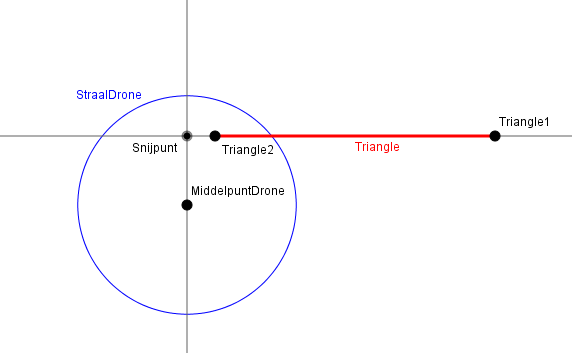
\includegraphics[width=1\textwidth]{Testbed/CollisionDetectionProbleem.png}
	\caption{Probleem met Collision Detection.\\ }
	\label{fig:CollisionDetectionProbleem}
\end{figure}